\section{Motivation}
The ability to measure changes in the hemoglobin concentration in skin has the potential to enable more personalized patient care which, in turn, could lead to an increase in treatment success rates and a decrease in per-patient costs. For example, in radiation therapy, a common side effect is a skin-reddening reaction known as erythema, or radiation dermatitis.\cite{McQuestion2006} Depending on the severity of the reaction, erythema can be quite painful and may even prevent the completion of the radiation treatment schedule, thereby reducing the overall treatment efficacy.\cite{Maciejewski1989} Although it is a deterministic effect, there is a varying threshold dose and a patient-dependent rate of increase in severity\cite{Hall2000} that makes erythema impossible to reliably predict in advance for an individual patient.\cite{Porock2002} Instead, patient responses are monitored by the therapy team over the course of treatment. Currently, the most prevalent method for monitoring erythema is by visual assessment (VA).\cite{McQuestion2006,Wong2013,Chan2014} VA uses a pre-determined scale to classify the current condition of the skin. If there are too few divisions on the scale (four or less), there is not a sufficient amount of information regarding the patient’s progress from the erythema stage to the next stage of moist desquamation. If there are more than four divisions on the scale, it is difficult to eliminate, or even minimize, the inter- and intra-observer variation, making the results imprecise. The implementation of a quantitative objective method for measuring skin redness could allow the treatment team to better manage the reaction, thereby potentially improving the treatment’s success rate and the patient’s quality of life.

Another application of a quantitative system for monitoring the hemoglobin concentration in skin is in the field of plastic surgery. Prior to incision, lidocaine (an anesthetic) and epinephrine (a hormone used for vasodilation) are commonly used to numb the surgical region and reduce bleeding during surgery. The commonly cited time to maximal effect of epinephrine is 7-10 minutes, but this time interval was determined in a porcine model\cite{Larrabee1987} in 1987 using laser Doppler flowmetry\cite{Swain1989} and was never confirmed with human trials or more advanced methods, possibly due to the associated difficulty and cost of the experiments.

Diffuse reflectance spectroscopy (DRS) with visible light (400-750 nm) is a good candidate for monitoring changes in the hemoglobin concentration in skin because the majority of these wavelengths of light do not penetrate deeper than the dermal layer.\cite{Richards-Kortum1996} As well, hemoglobin preferentially absorbs green light ($\sim550$ nm) and there are no major chromophores in the skin that absorb strongly in the red region ($\sim650$ nm).\cite{Prahl2001} The combined measurement and analysis techniques of DRS are many and varied,\cite{Palmer2006} but they can be categorized by whether the reflectance spectra are spatially resolved (at one or more radial positions from the source) or not.

DRS without spatial-resolution can be performed either with an integrating sphere or focusing optics, or with a bifurcated or random mixed fiber bundle.\cite{Stamatas2004} In both instances, the measured reflectance is interpreted as an analogue for the total diffuse reflectance but is not necessarily equal to it. For this reason, the majority of the analysis methods focus on using approximations to infer the hemoglobin concentration from the uncalibrated reflectance spectrum. Possibly the most popular approach is to relate changes in the area under the log-inverse-reflectance (LIR) spectrum to changes in the hemoglobin concentration. This approach was first proposed by Dawson et al. in 1980.\cite{Dawson1980} Dawson drew on work from chemistry in which the concentration of a chromophore could be determined from the transmitted light intensity through a sample cuvette using the Beer-Lambert law. He noted that when more hemoglobin was present, the area under the LIR curve increased, and he proposed an erythema index that was equal to the area under the curve (approximated by a polynomial) that represented the hemoglobin concentration in arbitrary units. Similar techniques have used the ratio between strategically chosen wavelengths (usually one green and one red) to act as a measure of the area under the LIR curve.\cite{Diffey1984,Lock-Andersen1998,Bodekaer2013} More recently, several researchers have shown a direct relationship between this area and the constituent chromophore concentrations.\cite{Stamatas2008,Kollias2010} However, due to the required assumptions and approximations made during this analysis, such as an unknown pathlength correction factor, the concentrations are still expressed in arbitrary concentration units and are incorrect should any of the non-hemoglobin concentrations change (e.g. melanin). A final method of analyzing this type of DRS measurement is by direct comparison with Monte Carlo simulations,\cite{Meglinski2002,Yu2008} but as it is computationally expensive and requires the obtained spectra to be highly characterized for modeling purposes, it is rarely used.

Presently available commercial systems that employ spatially-resolved DRS to determine the optical properties of human skin are limited to a fixed geometry fiber optic bundle, although video detection is possible. For a typical setup, several detection fibers are placed at one or more distances from the source fiber. The collected reflectance spectrum can either be fit with a model derived from diffusion theory or with the results of Monte Carlo simulations.\cite{Nishidate2011a} In either approach, the chromophore concentrations would act as fitting parameters. While both are capable of accounting for the layered structure of skin, the diffusion theory model fitting approach is less computationally expensive, and so is used most often.\cite{Zonios2001,Zonios2009,Reif2011,Tseng2012}

Recent advances in technology have made hyperspectral imaging (HSI) an option for detecting changes to the hemoglobin concentration in human skin.\cite{Yudovsky2010,Chin2012} An advantage to this technique is that it provides a spatial map of the hemoglobin concentration across the image instead of a ``single'' measurement location. However, as the technology is still relatively new, it is prohibitively expensive, and so is rarely used, especially outside of research institutions.

\section{Light-tissue interactions}
The propagation of light in tissue can be described by three main interactions:\cite{Niemz2007}
\begin{enumerate}
	\item Reflection (and refraction)
	\item Absorption
	\item Scattering
\end{enumerate}

Reflection and refraction occur at the boundary between two materials with different indices of refraction, such as between air and tissue. The light that is reflected at the boundary obeys the law of specular reflection which states that the angle of reflection of a ray of light is equal to the angle of incidence.\cite{Knight2013} Light that is transmitted past the boundary refracts toward or away from the normal as described by Snell's law,

\begin{equation}
n_1 \sin \theta_1 = n_2 \sin \theta_2
\end{equation}

\noindent where $n_1$ and $n_2$ are the indices of refraction of the two materials, $\theta_1$ is the angle of incidence, and $\theta_2$ is the angle of refraction.

The amount of light that undergoes either of these two processes can be predicted using Fresnel's equations which require the relative index of refraction ($n_2 / n_1$) and the angle of incidence ($\theta_1$) for input parameters.\cite{Pedrotti1993} There is a wavelength dependence in all indices of refraction that is negligible for small wavelength ranges.\cite{Doornbos1999,Knight2013}

While inside a material, light can either be absorbed or scattered. The probabilities of these two occurrences are based on the optical properties of the material. When an absorption event occurs, the light energy is transferred to a bound electron, elevating it to an excited state.\cite{Jacques2004} Atoms or molecules with excited electronic states can ``discharge'' this energy either through radiative processes such as fluorescence or phosphorescence or, more commonly, through non-radiative processes like vibrational relaxation. The probability of absorption occurring within an infinitesimal distance $ds$ is $\mu_ads$, where $\mu_a [mm^{-1}]$ is known as the absorption coefficient. In the case of (elastic) scattering, the exact process depends on the size of the particles with which the light interacts. When the particles are much smaller than the wavelength of light, Rayleigh scattering applies, which favors the scattering of shorter wavelengths in the forward or backward directions.\cite{Prasad2003} When the particles are comparable in size to the wavelength of light, Mie scattering best describes the interaction. Mie scattering is only weakly wavelength dependent and is forward-directed.\cite{Jacques2004} The probability of scattering occurring within an infinitesimal distance $ds$ is $\mu_sds$, where $\mu_s [mm^{-1}]$ is known as the scattering coefficient. 

Elastic scattering is isotropic in nature. However, in a medium with many small, suspended particles, another direction may dominate when Mie and Rayleigh scattering apply. This can be accounted for with an anisotropy factor ($g$) that is equal to the average cosine of the scattering angle. An anisotropy factor of $0$ represents isotropic scattering while a factor of $1$ represents forward scattering. To account for this directionality when modeling light transport in tissue, a reduced scattering coefficient is commonly defined as $\mu_s'=(1-g)\mu_s$ such that its inverse is the average distance between isotropic scattering events that would produce the same results as the anisotropic scattering.\cite{Gratton2004}

Another helpful quantity is the total reduced attenuation coefficient, $\mu_t'=\mu_a + \mu_s'$ which, when multiplied by an infinitesimal distance, represents the probability of any photon interaction occurring across that space. Its inverse is specially termed the ``reduced mean free path'' (mfp') and represents the average distance between interactions.\cite{Farrell2003}

\section{Modeling of light transport in turbid material}

\subsection{Radiation transport equation and diffusion theory}
The radiation transport equation (RTE), also known as the Boltzmann equation, describes the transfer of neutral particles (in this case, energy modeled as discrete photons) within an infinitesimal volume as a function of time.\cite{Duderstadt1976} It is often expressed as a change in the time- and space-resolved energy radiance, $L(\mathbf{r},\mathbf{\Omega},t)$ with respect to time. This quantity can be determined by investigating the mechanism by which the energy radiance can be gained and lost from the volume in question. When considering the steady-state condition, there is no net change in the energy radiance and the gain terms are equal to the loss terms.

\noindent The gain mechanisms are:
\begin{enumerate}
	\item Any photon sources within the volume, $ S(\mathbf{r},\mathbf{\Omega}) $
	\item Photons already within the volume that scatter into the direction of interest,  $\int_{4\pi} L(\mathbf{r},\mathbf{\Omega}) \mu_s(\mathbf{r},\mathbf{\Omega}' \rightarrow \mathbf{\Omega}) d \mathbf{\Omega'} $
	\item Photons that enter into the volume along the direction of interest
\end{enumerate}

\noindent Loss mechanisms include:
\begin{enumerate}
	\item Photons that are absorbed within the volume, $ \mu_a L(\mathbf{r},\mathbf{\Omega}) $
	\item Photons that scatter out of the volume, $ \mu_s L(\mathbf{r},\mathbf{\Omega}) $
	\item Photons that exit the volume
\end{enumerate}

\noindent A single convection term can be used to account for the photons entering and exiting the volume, $-\mathbf{\Omega}\cdot\nabla L(\mathbf{r},\mathbf{\Omega})$. The combination of all of the terms results in the following equation for the steady-state RTE,\cite{Farrell2003}

\begin{equation}
\label{eq:rte}
\mathbf{\Omega}\cdot\nabla L(\mathbf{r},\mathbf{\Omega}) + (\mu_a + \mu_s) L(\mathbf{r},\mathbf{\Omega}) - \int_{4\pi} L(\mathbf{r},\mathbf{\Omega}) \mu_s(\mathbf{r},\mathbf{\Omega}' \rightarrow \mathbf{\Omega}) d \mathbf{\Omega'} - S(\mathbf{r},\mathbf{\Omega}) = 0
\end{equation}

Solutions to the above equation may be found via intense numerical methods, but they are extremely computationally expensive to achieve. For this reason, a simpler approach is often employed in which approximations are made that simplify the RTE into a solution-friendly form. In the case of light transport in tissue, the diffusion approximation simplifies the above equation into a single differential equation. Diffusion theory requires: 1) that more scattering events occur than absorption events ( $ \mu_a < 0.1\mu_s'$), 2) that the radiance is, at most, linearly anisotropic, and 3) that the location of interest is sufficiently far from any boundaries (greater than 1 mfp).\cite{Jacques2004,Wilson2008} Under these conditions, the RTE can be reduced into the following diffusion equation,

\begin{equation}
\label{eq:diffeq}
\nabla^2 \cdot E(\mathbf{r}) - \frac{\mu_a}{D}E(\mathbf{r}) = S(\mathbf{r})
\end{equation}

where $E(\mathbf{r})$ is the energy fluence rate (the integral of the energy radiance over all angles), $D$ is the diffusion constant, $(3\mu_t')^{-1}$, and $S(\mathbf{r})$ is the source term.

The diffusion equation can be solved analytically by applying a set of boundary conditions. In the case of tissue optics, the most common sets of boundary conditions, such as the extrapolated boundary condition, attempt to satisfy the Robin boundary condition through various approximations with image sources and extended boundaries.\cite{Prahl1995}

\subsection{Monte Carlo simulations}
\label{sec:mc}
Monte Carlo (MC) simulations offer a method of solving the steady-state RTE that is slightly less computationally expensive than traditional numerical methods. It is also useful for confirming solutions for approximations such as diffusion theory. Millions of photons are ``launched'' and their propagation through the medium is determined by the random sampling of probability distributions that represent the absorption and scattering conditions of the medium. The basic principles of MC simulations have been thoroughly covered by Prahl \emph{et al.}\cite{Prahl1989} and Wang \emph{et al.},\cite{Wang1995} so only two important variations are outlined here.

If a single simulation must be run several times with different sets of optical properties, it is useful to adapt the code into what has been termed mono (or “white”) MC.\cite{Kienle1996a,Alerstam2013} Under this simulation, photons are tracked through a homogeneous scattering, non-absorbing medium. There is no survival weighting in mono MC, so the photons' weights are never modified in the tissue and they are only killed when they scatter too many times (via Russian roulette) or migrate too far from the region of interest. The total distance traveled by each photon (the pathlength, $s$) in the medium is tracked. When photons are finally scored, their weight is added to a bin for the corresponding total pathlength. The effect of absorption can be introduced after the simulation is complete by multiplying each bin by $\exp(-\mu_as)$ and summing over all the bins.

When multiple processors are available on a computer, parallelization is an option for increasing the speed of the MC simulation. In parallel computing, single calculations are performed by each available processor in a computer and the results are collated at the end. Parallelization is only possible if all the calculations are independent of one another (i.e. the order doesn't matter). Since MC is based on stochastic processes, each photon can be treated separately. For example, in a computer with four processors, it is possible to track four photons simultaneously, record their progress, and collect their results once terminated. This yields a MC simulation that would run four times faster than the original serial code.

\section{In vivo measurements of tissue optical properties with diffuse reflectance}
\label{sec:diff_refl}
For the purposes of monitoring patient response, \emph{ex vivo} methods of DRS for determining tissue optical properties are obviously not appropriate. Therefore, this section will focus solely on \emph{in vivo} methods, specifically those that require steady-state conditions.

\subsection{Total diffuse reflectance}
\label{sec:total_diff_refl}
The total diffuse reflectance represents the fraction of incident light fluence remitted from the tissue across the entire surface (i.e. it is spatially integrated) at a single wavelength. It can be modeled with the diffusion approximation and is dependent only on the reduced albedo and the relative index of refraction.\cite{Kim2011} The index of refraction for skin has been accurately measured, and a value of 1.4 is typically used for incident light within the visible spectrum.\cite{Kienle1996a} With this information, the albedo of the tissue can be determined from the measured total diffuse reflectance. For a single total diffuse reflectance measurement, there is no way to determine the individual contributions from scattering and absorption. However, if the scattering and mean pathlength are assumed constant, a second measurement in which the absorption coefficient is known or can be approximated, will allow for the determination of the first absorption coefficient. This technique relies on the relationship between the total diffuse reflectance and the exponential of the product of the absorption coefficient and the pathlength,

\begin{equation}
	R_d\propto\exp\left(\mu_al\right)
\end{equation}

 \noindent The total diffuse reflectance is generally measured either with an integrating sphere (see Section~\ref{sec:is_theory}) or with an optical system, off-set from the normal to avoid collecting any specular reflectance.

\subsection{Spatially-resolved diffuse reflectance}
\label{sec:spat_diff_refl}
The spatially-resolved diffuse reflectance is the fraction of the incident light remitted at a set of radial distances from the incident light source. It can be collected in one of two ways: either with an imaging system\cite{Kienle1996b} or by detection fibers positioned at known distances from the source fiber.\cite{Kim2011} In a fiber optic array, the source and detection fibers are usually bundled together in a single probe to maintain accurate and consistent positioning of the fibers. Several detection fiber probes are used at greater distances to improve the signal-to-noise ratio (see Figure~\ref{fig:intro-srdr}). The signals from the detection fibers are then processed by a spectrometer. When the reflectance is captured with an imaging system, such as a digital camera, the radially-dependent reflectance curve can be constructed by binning pixel intensities at equal radial distances. This method provides more data points for the subsequent analysis. Unless a hyperspectral camera is used, only the optical properties at a single wavelength (that of the incident laser source) can be determined.

\begin{figure}
	\centering 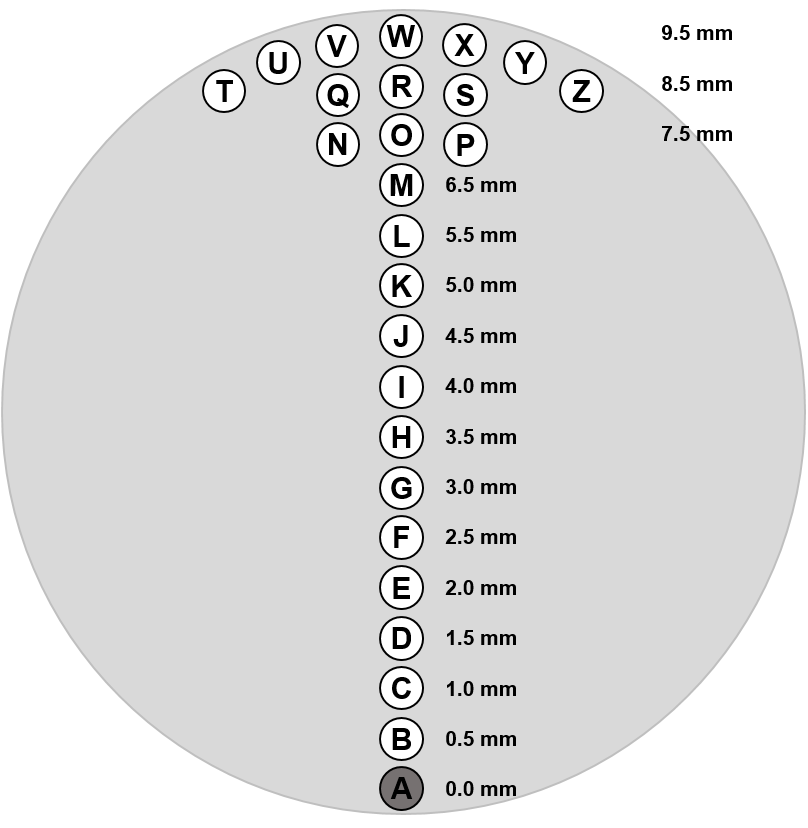
\includegraphics[width=0.5\textwidth]{figures/intro-srdr.png}
	\caption[Probe for spatially-resolved diffuse reflectance]{\label{fig:intro-srdr}A diagram representing the configuration of the optical fibers in a spatially-resolved diffuse reflectance probe. Light enters through fiber “A” (dark grey) and is detected by additional fibers placed at set distances away (white). More fibers are placed at further distances to strengthen the signal.}
\end{figure}

Both the absorption and reduced scattering coefficients can be determined from this collected data. One analysis method is to compare the spatially resolved diffuse reflectance spectrum to one produced by a single mono Monte Carlo simulation. In addition to applying the effect of absorption post-simulation (see Section~\ref{sec:mc}), it is also possible to scale the results for different scattering coefficients from a single reference scattering coefficient as follows,\cite{Kienle1996a}

\begin{equation}
	R(\rho) = \left(\frac{\mu_s'}{\mu_{sref}'}\right)^2 R_{ref}\left(\rho\frac{\mu_s'}{\mu_{sref}'}\right)
\end{equation}

\noindent where the ratio of the new reduced scattering coefficient to the reference reduced scattering coefficient acts as a scaling factor. A fitting algorithm will adjust the optical properties and generate a reflectance curve from the MC data until the resulting chi-squared statistic between the measured data and the calculated data is minimized.

The data can also be fitted with a nonlinear equation for the spatially-resolved reflectance derived from diffusion theory. The absorption and reduced scattering coefficients would act as input parameters for the equation and those that resulted in the best fit (via a given fitting algorithm) would be the approximate values. When deriving this equation, the selection of the boundary conditions is integral in recovering reliable results. Farrell \emph{et al.}\cite{Farrell1992} used an extrapolated boundary condition and an negative image source to yield a fluence rate of zero at a new (extrapolated) boundary located above the actual tissue-air interface. The height of the image source and the boundary are dependent on the tissue optical properties. Using this set of approximations and boundary conditions, the recovered values for the absorption and reduced scattering coefficients agreed with the true values within 10\%.

%\begin{equation}
	%R(r) = \frac{1}{4\pi}\left[z_0 \left(\mu_{eff} + \frac{1}{\rho_1}\right) \frac{e^{-\mu_{eff}\rho_1}}{\rho_1^2} + \left(z_0 + 2z_b\right) \left(\mu_{eff} + \frac{1}{\rho_2}\right) \frac{e^{-\mu_{eff}\rho_2}}{\rho_2^2}  \right]
%\end{equation}

\subsection{Spectrally-constrained diffuse reflectance}
\label{spec_diff_refl}
The most common method employs a single source-detector pair instead of a spatially-resolved array of detector fibers. In this approach, a broad spectrum light source is used instead of a single wavelength light source, and the collected signal is resolved into a reflectance measurement at each wavelength. However, this reflectance spectrum is not sufficient to determine the tissue optical properties. Generally, a forward model of the diffusion theory is derived and fit to the obtained reflectance spectrum. Such a model requires both the absorption and reduced scattering coefficient spectra, which can be approximated.

The absorption coefficient is estimated to be the sum of the individual chromophore concentrations $c_i$, multiplied by their respective extinction coefficient spectra $\varepsilon_i(\lambda)$, as follows,

\begin{equation}
\mu_a(\lambda) = \sum_i c_i \varepsilon_i(\lambda)
\end{equation}

The extinction coefficient is the absorption coefficient per molar ($mol/L$) for the medium. These spectra for the majority of chromophores found in human skin (see Section~\ref{sec:skin}) have been well characterized and the chromophore concentrations are included as fitting parameters in the forward model. It is important to include only those chromophores that contribute significantly to the overall absorption within the wavelength range of interest.\cite{Kim2011} Including insignificant chromophores will add too many variables to the fitting equation while omitting significant chromophores will yield inaccurate results.

The reduced scattering coefficient for human skin has been well-characterized and follows a wavelength-dependent power law,\cite{Doornbos1999}

\begin{equation}
\mu_s'(\lambda) = a\lambda^{-b}
\end{equation}

As a result, the scaling factor $a$, and the exponential $b$ can be included as fitting parameters in the forward model. This spectrally constrained approach has been used by Yohan et al.\cite{Yohan2014} where it was used to track ionizing radiation-induced erythema through the hemoglobin fitting parameters.

\subsection{Commercially available systems}
Currently available commercial systems that measure diffuse reflectance are primarily used in dermatological applications. As such, their focus is on measuring the skin color which is directly related to the concentrations of the chromophores found in skin, specifically oxy- and deoxy-hemoglobin, and melanin.

Two such systems are the DSM II Skin ColorMeter (Cortex Technology, Hadsun, Denmark) and the Mexameter\textregistered MX 18 (Courage+Khazaka electronic GmbH, Cologne, Germany). The DSM II Skin ColoMeter employs a plastic probe with focusing optics to shine a white LED onto the skin surface. The reflected light is then focused back onto multispectral detectors within the probe. The detector processes the reflected signal into one of the many color systems (RBG, CMYK, or L*a*b*) or a proprietary erythema index. The Mexameter uses three wavelengths (568 nm, 660 nm, and 870 nm) emitted by a 16 LED array onto the skin within a probe head that is placed on the skin surface. The requirement of direct contact between the skin and the probe suggests that this may be a fiber-based device although that is not explicitly stated. The red and near-infrared (NIR) wavelengths are used to determine a melanin index, and the green and red wavelengths are used to determine the erythema index.\cite{Clarys2000} Both systems rely on calibration measurements performed on black and white reflectance standards (provided).

The prices for either system could not be determined from the company websites, but a recent competitor, the Derma Spectrometer (MIC Global, London, United Kingdom) (no longer for sale) was priced at \$6000 in early 2014.

\section{Integrating sphere theory}
\label{sec:is_theory}
An integrating sphere is a light delivery and/or collection device. As its name suggests, it is made from a hollow sphere with several ``ports'' cut out of the surface through which light can enter or exit. A typical sphere is shown in Figure~\ref{fig:intro-is_sample}. The inner surface of the sphere is covered with a highly diffuse reflective coating to create what is known as a Lambertian surface. When used as a light delivery device, the light emitted from the irradiation port is uniformly distributed and is isotropic in direction. When used as a measurement device, it is capable of capturing all of the light emitted from the sample area directly below the measurement port. Together, these illumination and measurement qualities make integrating spheres ideal for measuring the total diffuse reflectance (spectrum).

\begin{figure}
	\centering 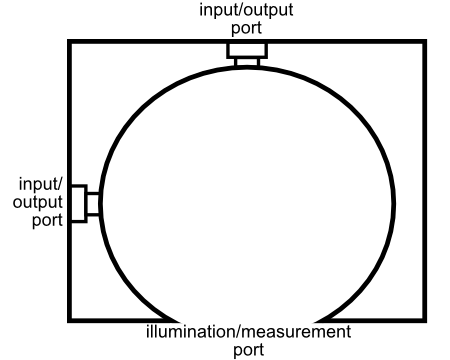
\includegraphics[width=0.5\textwidth]{figures/intro-is_sample.png}
	\caption[Sample integrating sphere diagram]{\label{fig:intro-is_sample}A diagram displaying a common geometry for an integrating sphere. There are two ports for delivering and collecting the light and one port for measuring the reflectance from a sample.}
\end{figure}

\subsection{Relative reflectance and sphere throughput}
The total diffuse reflectance is a relative (as opposed to absolute) reflectance measurement. As such, it requires a characterized reflectance sample known as a reference standard. Measurements performed with the sample of interest are compared to measurements performed with the reference standard. To ensure accurate reflectance measurements, it is important to maintain a consistent throughput, or efficiency within the sphere between the sample and the standard measurements.\cite{Hanssen2002}

The throughput or efficiency of an integrating sphere is the best way of characterizing its performance. It can either be empirically determined or approximated by the following equation,

\begin{equation}
\tau = f_d \frac{\rho_w}{1-\bar{\rho}_w}
\end{equation}

\noindent where $f_d$ is the exchange factor -- equal to the ratio of the total surface area of all the ports to the surface area of the sphere, $\rho_w$ is the actual reflectance of the sphere wall material, and $\bar{\rho}_w$ is the average sphere wall reflectance accounting for the reflectances at each of the ports.

When the integrating sphere is sufficiently large, a change in the reflectance at one of the ports has a proportionately small effect on the sphere's throughput. Unfortunately, large spheres are not only expensive, but often impractical. For smaller spheres, changes in the sphere throughput between the sample and the reference standard cause what are known as Single Beam Substitution Errors (SBSE) in the total diffuse reflectance measurement.

If the sphere is sufficiently large to allow for an additional ``dummy'' port, a second measurement can be performed to account for SBSE, as shown in Figure~\ref{fig:intro-is_compar}.\cite{Labspherec} The geometry for the first measurement positions the sample directly opposite the light source and the reference standard at the dummy port. This is the primary reflectance measurement. The geometry for the second measurement positions the reference standard directly opposite the light source and the sample at the dummy port. This represents the background correction factor. Under this experimental design, the sphere throughputs and average reflectances are equal for the two measurements.

\begin{figure}
	\centering 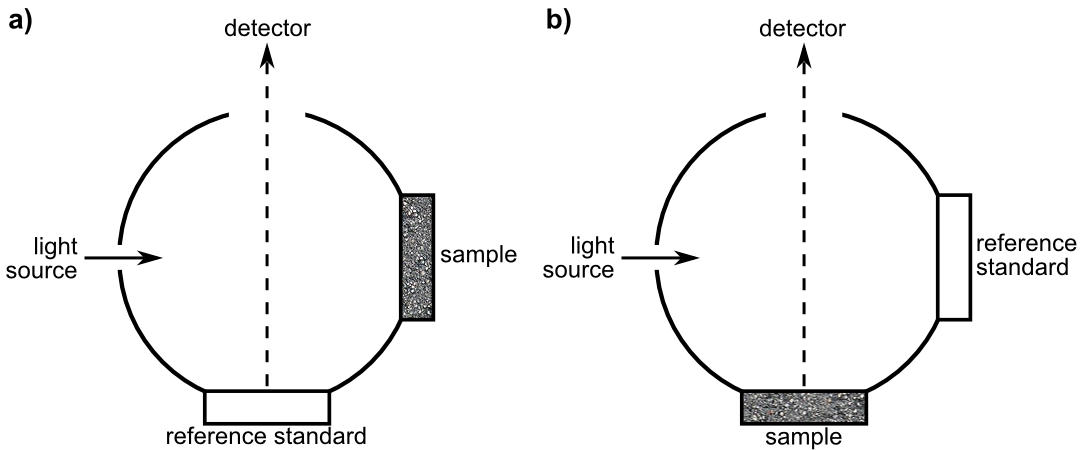
\includegraphics[width=1.0\textwidth]{figures/intro-is_compar.png}
	\caption[The comparison method for measuring sample reflectance]{\label{fig:intro-is_compar}To ensure a constant throughput in the sphere between sample and reference measurements, a dummy port can be added to sufficiently large spheres that will eliminate the SBSE.}
\end{figure}

If the sphere is too small to permit a second port, the SBSE must be corrected mathematically or empirically. Of these two options, the empirical approach is preferred as a mathematical solution would be extremely complex and only accurate if precise values for parameters such as port fractions and reflectances were provided. For a given sphere, reflectance measurements are performed on a set of characterized reflectance standards covering the range of reflectances expected from the unknown samples. By comparing the observed reflectances to the expected ones, a correction factor equation or a lookup table can be produced. This process is described in detail in Chapter~\ref{chap:p1-system}.

\subsection{Integrating sphere design}
When constructing an integrating sphere, there are several major design parameters that must be optimized to minimize measurement error. The first is the sphere size, which cannot be determined until the total surface area of all of the ports has been calculated. Ports intended for coupling with optical fibers will have a fixed surface area while the area of the detection/illumination port(s) will depend on the use of the sphere. Once the total surface area of the ports has been determined, the sphere size can be calculated based on the rule of thumb that the resulting exchange factor be less than 5\%.\cite{Labsphereb} Spheres that exceed this ratio no longer display some of the desired characteristics such as the isotropy of the light within the sphere.

The next consideration is the material of the sphere wall or the sphere's internal coating. Spheres can be created from a highly reflective material such as Spectralon\textregistered, or they can be produced with another material and subsequently coated on the inside with a highly reflective paint, such as barium sulfate. In either case, it is extremely important that the interior surface of the sphere have as high a reflectance as possible, ideally greater than 94\%. This material should also be matte or diffuse in nature in order to produce the desired scattering that creates the isotropic illumination.

The final consideration for the integrating sphere is the geometry of the ports. Usually light from the input port is not directly incident on the output port. To accomplish this, the numerical aperture of the optical fibers connected to the ports and the overall sphere geometry should be considered. If physical positioning of the ports cannot accomplish this task,  wall projections into the center of the sphere, known as baffles, can be added. Baffles are not ideal for smaller spheres as they introduce inhomogeneities to the smooth inner surface of the sphere that affect the isotropic characteristic. Once this requirement has been satisfied, the illumination geometry can be decided. The two most popular setups are: (1) diffuse-direct (d/0\degree), where incident light is first incident on the sphere wall and the detection port is directly opposite the output port, and (2) direct-diffuse (0\degree/d), where the incident light is first incident on the detection port and the output port is focused on a portion of the inner sphere wall.\cite{Springsteen1998}

\section{Human skin}
\label{sec:skin}

\subsection{Skin Anatomy}
Human skin consists of three main layers: the epidermis, the dermis, and the subcutaneous layer.\cite{Fodor2011a} The epidermis is the top-most layer of skin. Keratinocytes (skin cells) are produced at the deepest section of the epidermis in the stratum basale (or basal layer) and migrate toward the surface, through the statum spinosum and the stratum granulosum to the stratum corneum, losing their internal structures and organelles during the process (see Figure~\ref{fig:intro-skin_layers}). Once the cells reach the skin surface, they are no longer alive and can be shed easily. The basal cells undergo mitosis at an average rate of 10\% per day\cite{McQuestion2006} and the migration of cells toward the surface occurs at a steady equilibrium rate. A completely new dermal layer is formed every 4 weeks. Also found in the epidermis are melanocytes, the melanin-producing cells which are majorly responsible for skin color. The average epidermal thickness is 0.1 mm.\cite{Yang2009}

\begin{figure}
	\centering 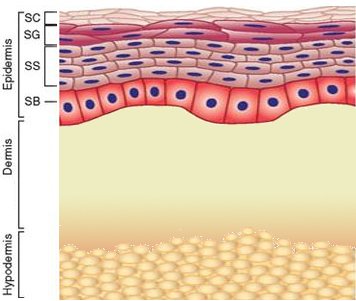
\includegraphics[width=0.5\textwidth]{figures/intro-skin_layers.jpg}
	\caption[Cross-section of layers of human skin]{\label{fig:intro-skin_layers}The three main layers of skin: The epidermis, the dermis, and the subcutaneous layers. Cells of the epidermis begin at the stratum basale (SB) and migrate through the stratum spinosum (SS) and stratum gradulosum (SG) to the stratum corneum (SC). Modified with permission: \textcopyright David J. Wong (\url{http://www.stembook.org}), \href{http://creativecommons.org/licenses/by-sa/3.0/}{CC-BY-SA-3.0}.\cite{Wong2009}}
\end{figure}

The second layer of skin is the dermis. It contains mostly collagen and elastin fibers but is also the location of capillaries and some nerves. The average dermal thickness is approximately 1.5 mm but can vary widely depending on the site.

Below the skin is the subcutaneous layer, also known as the hypodermis or subcutis. The thickness of this layer varies greatly because this is the layer that contains subcutaneous fat. This is also the location of the majority of superficial veins which can occasionally be visible at the surface. A representative thickness for this layer is 5 mm.

Light in the visible spectrum (400-750 nm) is only able to penetrate the first two layers of skin.\cite{Kochevar2012a} For 500 nm light (green/blue), the average penetration depth in human skin is 0.6 mm while for 700 nm light (red/near-infrared), the average depth is 1.2 mm.\cite{Richards-Kortum1996} Diffusely reflected light must first travel into and then out of the skin, therefore the majority of the reflected light signal is due to scattering and absorption events within the epidermis and dermis. Within these layers, the dominant chromophores are: oxy- and deoxy-hemoglobin, and melanin. The relative extinction coefficient spectra for these three chromophores are shown in Figure~\ref{fig:intro-skin_chromophores}. While water accounts for roughly 70\% (w/w) of human tissue,\cite{Nakagawa2010} its absorption below 700 nm is negligible. Similarly, beta-carotene (in the epidermis) and bilirubin (in the dermis) do not contribute significantly at wavelengths above 450 nm. Also, they are only found in relatively small concentrations in healthy human skin. Although its contribution is small, there is a significant amount of absorption by the structural components of skin.\cite{Bargo2005}

\begin{figure}
	\centering 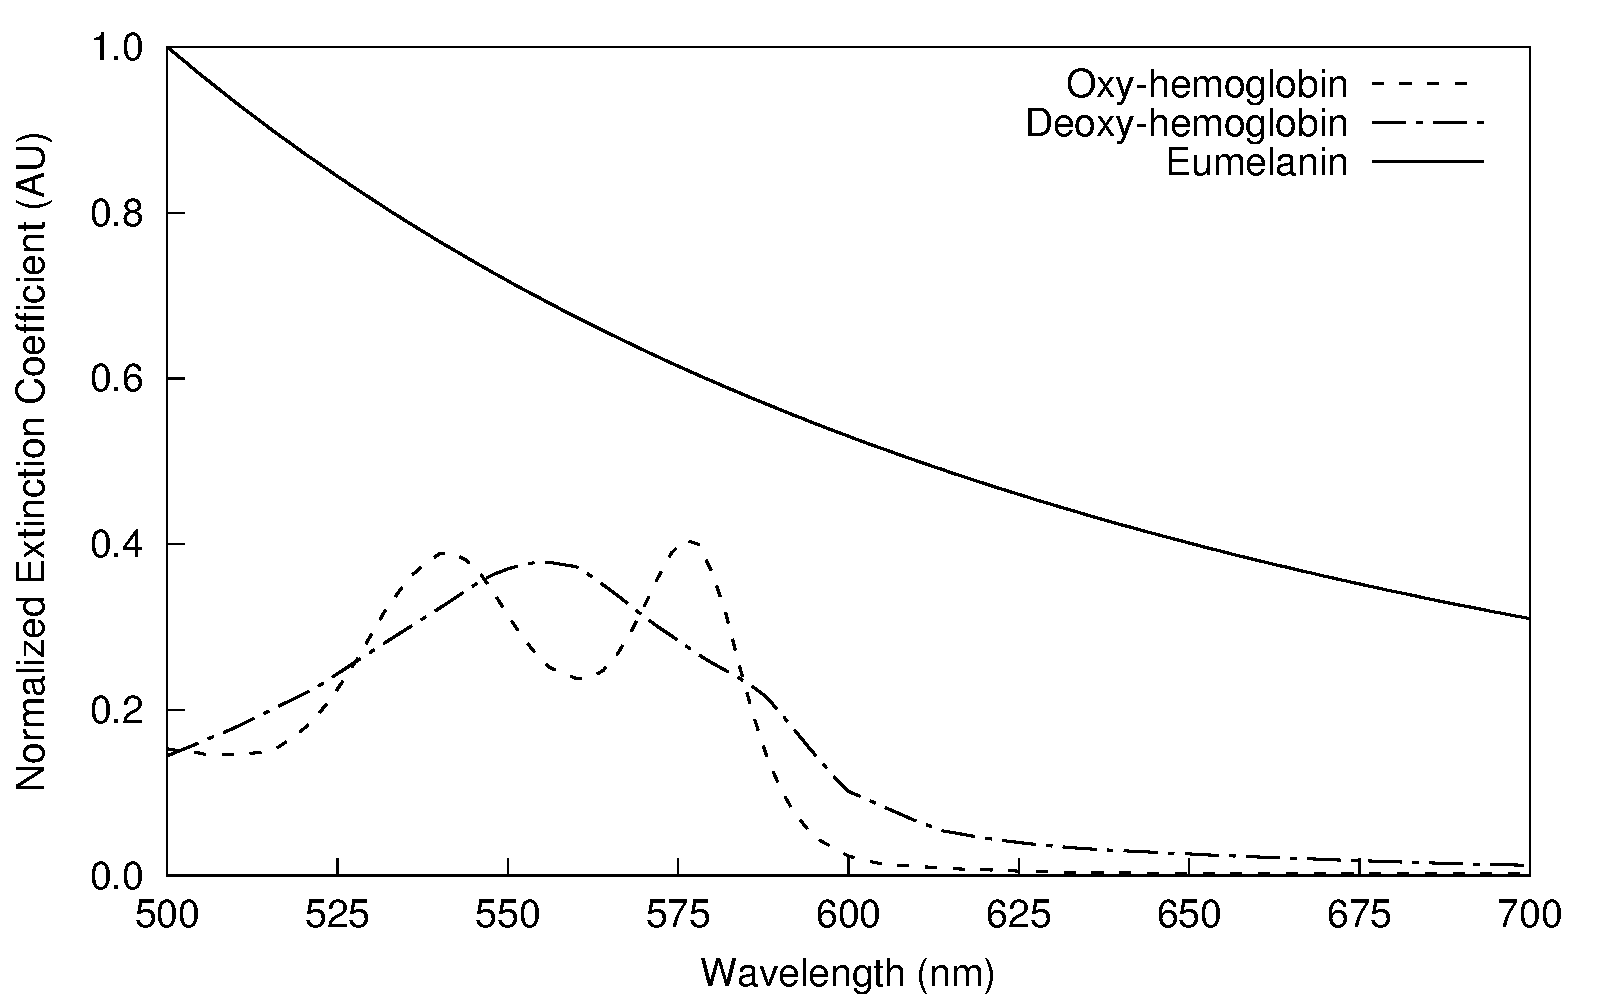
\includegraphics[width=0.6\textwidth]{figures/intro-skin_chromophores.png}
	\caption[The extinction coefficient spectra for the major chromophores of skin within the visible light spectrum]{\label{fig:intro-skin_chromophores}The extinction coefficients of the major chromphores found in skin within the visible light spectrum: Oxy- and deoxy-hemoglobin and melanin. Data shown are from Prahl \& Jacques (2001).\cite{Prahl2001}}
\end{figure}

\subsection{Skin Physiology}
Changes to the vasculature within the dermal and subcutaneous layers impacts the blood flow that, in turn, changes the physical appearance at the surface. When the blood vessels narrow, less blood is present in the dermal layer of the skin. This process is known as vasoconstriction and results in a perceived blanching of the skin. When the blood vessels expand in a process known as vasodilation, more blood is present in the skin, which appears redder to the human eye.

As illustrated in Figure~\ref{fig:intro-skin_chromophores}, both oxy- and deoxy-hemoglobin have low absorption in the red region of the visible spectrum, but have significant absorption within the green/yellow region. Therefore, when vasodilation occurs, the skin does not appear redder due to an increase in reflected red light, rather it is because of a decrease in the other colours in the reflected spectrum. Similarly, when vasoconstriction occurs, more green and yellow light are scattered back out of the tissue, contributing to a whiter appearance given that white light is a collection of all of the colors within the visible spectrum. Regarding the ratio of the two major hemoglobin chromophores during these two processes, McNaulty \emph{et al.} determined that the tissue oxygen saturation ($StO_2$) is related to blood flow.\cite{McNulty2011} Therefore, more oxy-hemoglobin is present during vasodilation and less is present during vasoconstriction.

Vasoconstriction and vasodilation are normal thermal regulatory responses of the human body.\cite{Kellogg2012} When the body begins to overheat, blood vessels near the surface expand to release heat. When the body temperature drops, blood vessels in the skin constrict to maintain more blood flow in the core. While this is the most commonly observed cause of these two processes, both can be induced by other means. For example, the anesthetic lidocaine acts as a vasodilator and epinephrine, a hormone, behaves as a vasoconstrictor. They are often used together in a subcutaneous injection to simultaneously numb the region of interest while keeping it blanched for better viewing and minimal bleeding during surgery. As the name suggests, the needle is inserted into the subcutaneous tissue below the dermis and acts on the blood vessels that span both layers. The actual area of skin impacted depends on the volumes and concentrations of the two injected drugs. Depending on the local vasculature, the effect can last up to several hours.

Vasodilation is also the most common response to inflammation because the increased blood flow supplies the affected tissue with more oxygen and white blood cells, which are useful when infection occurs. During radiation therapy, radiation dermatitis/erythema occurs because some of the healthy cells in the basal layer are prevented from dividing.\cite{Fitzgerald2008} This disrupts the steady rate of progression of cells toward the skin surface, causing an inflammatory response.\cite{Simonen1998} Erythema is also promoted by an increase in skin dryness due to the destruction of sweat and oil (sebaceous) glands. Although all patients respond differently and are prescribed different treatment plans, the general trend is for erythema to appear around the second week of treatment and last for approximately two to four weeks following treatment. For head and neck intensity modulated radiation therapy (IMRT), clinical experience predicts that the maximum skin response will occur during the fifth week of treatment (J. Wright, personal communication, Aug. 28, 2014.).

\section{Thesis proposal}
Currently available commercial systems for monitoring erythema rely on total diffuse reflectance spectroscopy.\cite{Clarys2000} As a result, they can only provide measurements in the form of a skin redness scale (or ``erythema index''). Such an index is only capable of detecting when skin is more or less red compared to some baseline measurement, and it cannot account for changes in non-hemoglobin chromophores.

Other clinical systems rely on a spatially-fixed spectrally-constrained diffuse reflectance approach.\cite{Kim2010} Such systems are capable of accounting for changes in the non-hemoglobin chromophores but may be more sensitive to positioning errors compared to an integrating sphere-based system.

A combination of the two approaches will result in a user-friendly system capable of accounting for all chromophore concentration changes. Thus, a spectrally-constrained model to interpret the total diffuse reflectance spectra obtained with an integrating sphere is proposed. Similar systems have been built by Yudovsky and Pilon,\cite{Yudovsky2010a,Yudovsky2011} but their derived model was tested on data measured in 1952, and since they did not account for integrating sphere effects, their model did not fit well to the data, particularly outside of the hemoglobin feature wavelengths. As such, careful consideration should be paid when building and characterizing a similar system. In Chapter~\ref{chap:p1-system} of this thesis, a paper is presented that outlines the elements of such a system and how its response was characterized. In Chapter~\ref{chap:p2-mckee}, the system, combined with a standard erythema index, was used to determine the time to maximal effect of epinephrine. In Chapter~\ref{chap:p3-model}, a paper proposing a spectrally-constrained model for interpreting the spectra obtained with the established system is presented. Special consideration is paid to the necessary corrections required when the total diffuse reflectance spectrum is collected instead of the standard fixed-position diffuse reflectance spectrum. The system and model are then combined in Chapter~\ref{chap:p4-imrt_study} and used to monitor the skin redness of patients undergoing IMRT for cancers of the head and neck. The results are used to outline the proper implementation of quantitative analysis in a study comparing two treatment interventions or management regimens. Such additional consideration is necessary due to the large daily variation in the hemoglobin concentration in skin. Along with the skin redness measurements, weekly TLD readings were performed to confirm the skin dose in the measurement region. These data were later used to determine TLD placement and positioning reproducibility in Chapter~\ref{chap:p5-tlds}.